\renewcommand{\figurename}{}
\mychapter{Préparation de la solution de communication client}{cap:preparation_itop} 
\lhead{Préparation de la solution de communication client}

La phase d'étude la nouvelle solution de support s'est terminée la période dernière. Le choix s'est arrêté sur Combodo iTop, qui fut mis à l'épreuve dans un environnement contrôlé, répondant au mieux au cahier des charges et aux tests effectués.
\\ \\
L'objectif de cette troisième période est d'en faire la nouvelle interface de communication client, en basculant les informations présentes de l'ancienne interface, et en l'aménageant selon nos besoins et les retours pour un lancement présumé la période d'alternance prochaine.

\section{Mise en relation des connaissances et des documents clients}

Une première étape dans l'installation de la solution a été la mise en commun et à jour des informations clientes pour avancer vers une plateforme saine et actuelle. Ainsi, en ne renseignant auprès de nos clients, de mes collègues puis des factures : j'ai rassemblé beaucoup d'informations pour avoir une base fraîche d'informations clients à utiliser pour la nouvelle solution.
\\ \\
Ainsi ont été mis à jour les membres et les services que proposent nos clients, les services que nous leur proposons, leurs contacts informatique et les notres chez eux, les emplacements de leurs sites etc. J'ai organisé les données pour qu'elles soient réutilisables pour être manipulées dans d'autres projets futurs facilement.
\\ \\
À l'issue de cet exercice, j'avais toutes les informations à renseigner dans la nouvelle interface afin que nos clients n'aient pas d'informations erronées ou qu'ils aient à les renseigner eux mêmes.

\section{Première communication du changement aux clients}

Avant le déploiement de la solution, il est capital d'avertir nos clients du changement de l'interface de support. La communication est lourdement importante, peu importe la criticité du service touché : nos clients ne doivent pas être pris au dépourvu ou se questionner sur nos activités ou à l'utilisation d'un service.
\\ \\
Avec mon tuteur Guillaume et mon responsable Éric, nous avons envoyé un premier courriel informant du changement de l'interface futur, comment ce basculement allait procéder, et des avantages que nos clients en auraient - pour toujours les tenir informer de notre activité.
\\ \\
Un email de rappel a aussi été envoyé la semaine en suivant, s'en est suivi d'un troisième pour leur transférer leurs identifiants de connexion la veille du lancement.

\section{Inspections et modifications après absence}

La première approche technique à mon retour a été d'observer si les fonctionnalités implémentées la période dernière étaient toujours fonctionnelles et stables, pour les corriger avant le déploiement si nécessaire.
\\ \\
La fonctionnalité de création d'une demande ou d'un incident par courriel était manquante, fonctionnalité que je n'ai pas corrigée par contrainte de temps et pour son importance basse (pour les activités que j'avais à faire)..
\\ \\
Durant cette période, j'ai aussi appliqué des modifications dans le cadre du déploiement dans un milieu de production, majoritairement de sécurisation et de renforcement du système d'informations et de ses communications pour limiter son exposition (informations susceptibles d'être utilisées pour de la recherche de vulnérabilités).

\subsection{Tests de fonctionnement}

Dans un deuxième temps, j'ai effectué des essais pour simuler une interaction client - ADITU pour s'assurer du bon fonctionnement de l'ensemble, même dans des cas particuliers.
\\ \\
Une notion complexe de cet exercice fut d'illustrer l'intuition que pouvait avoir un client en utilisant une interface sans considérer nos aspects acquis de navigation sur Internet (sans avoir les mêmes connaissances ou compréhension que nous dans l'utilisation d'outils informatique...).
\\ \\
Nous en sommes venu à en vouloir simplifier l'interface, les clients voulant que ce soit simple et rapide pour reprendre leur activité au plus vite. Ainsi, elle se résume en un ensemble d'étiquettes cliquables, avec des intitulés et des descriptions.
\\ \\
En voici quelques illustrations à l'arrivée du client sur l'interface.

\begin{figure}[H]
    \centering
    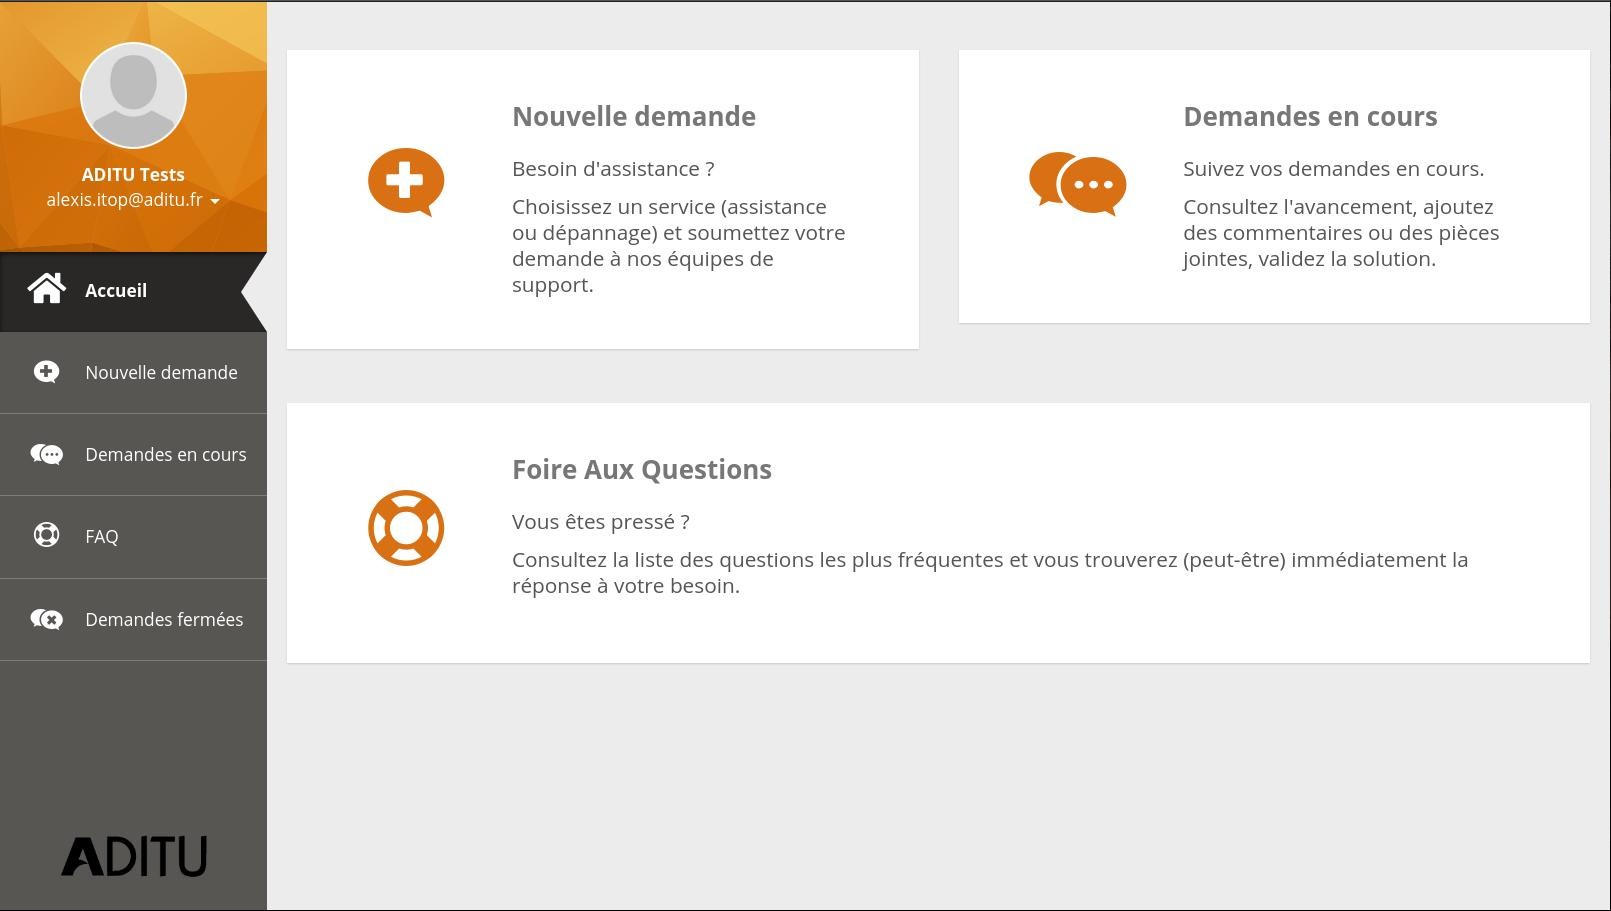
\includegraphics[width=\textwidth - \textwidth / 10]{ressources/images-itop/00.jpg}
    %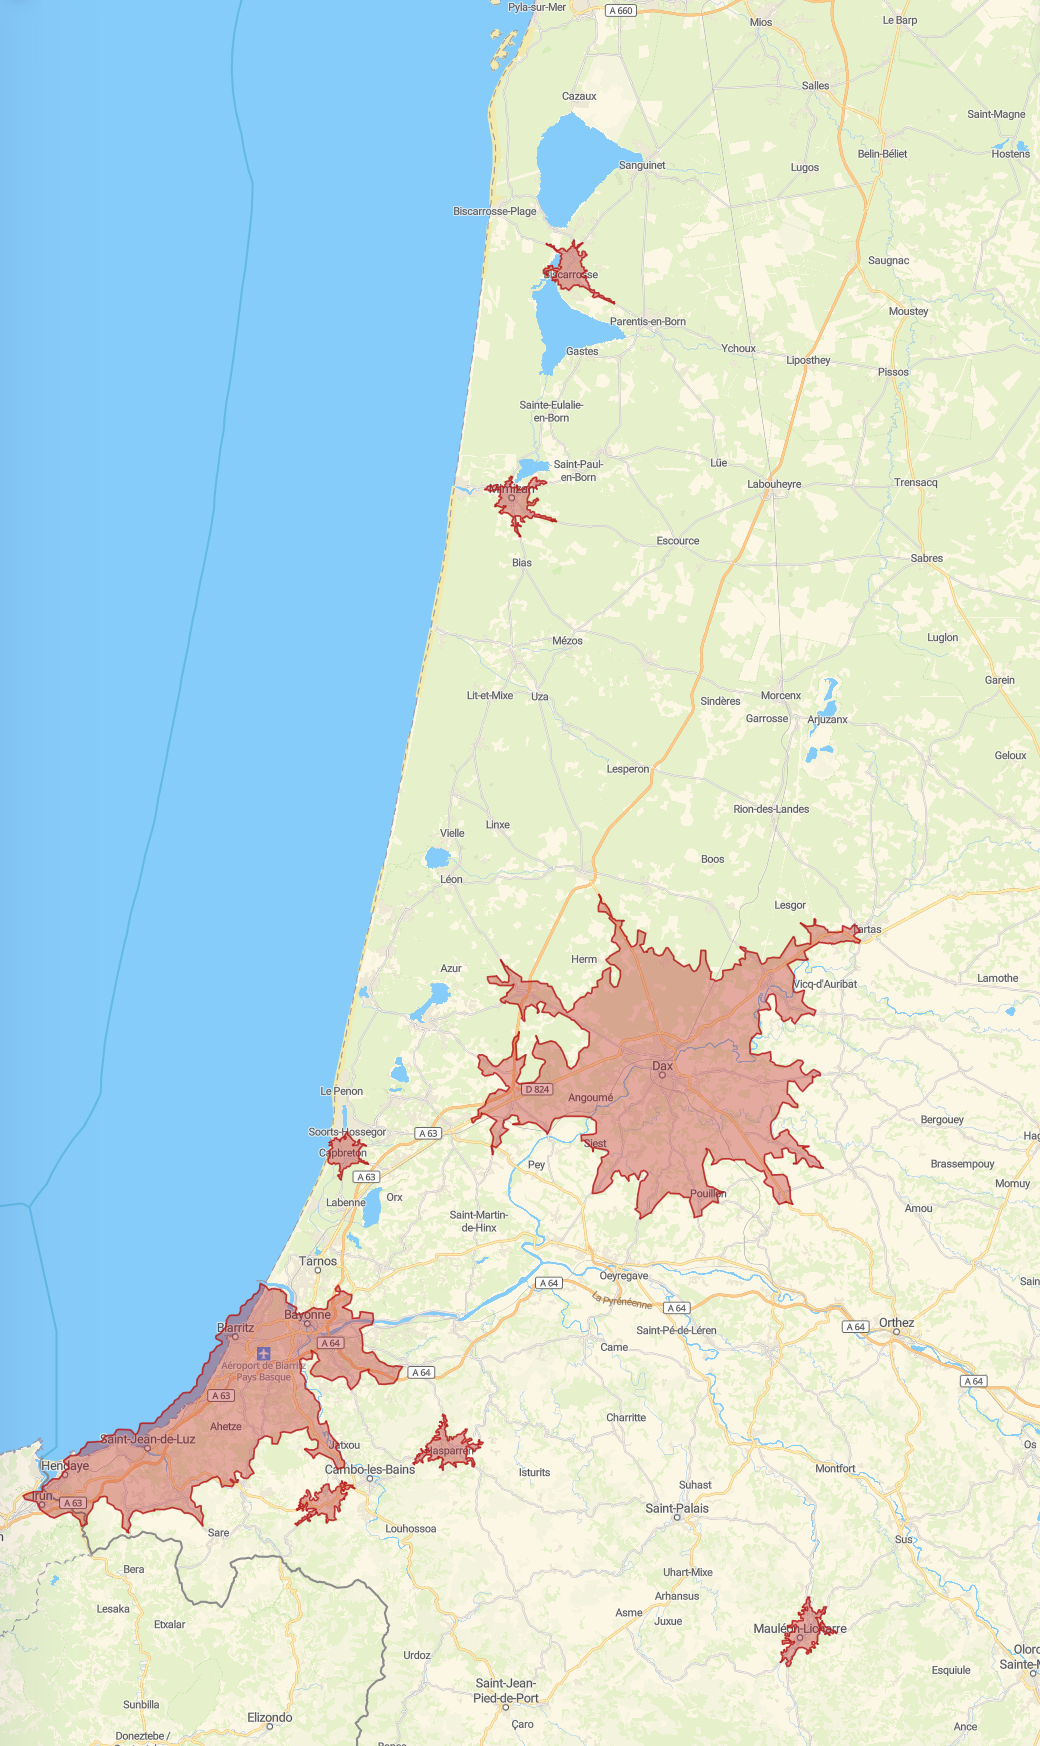
\includegraphics[scale=0.2]{zone_chalandise_aditu.png}
    \figurename
    \caption{Arrivée du client sur l'interface de support}
    \label{fig:00-itop}
\end{figure}

\begin{figure}[H]
    \centering
    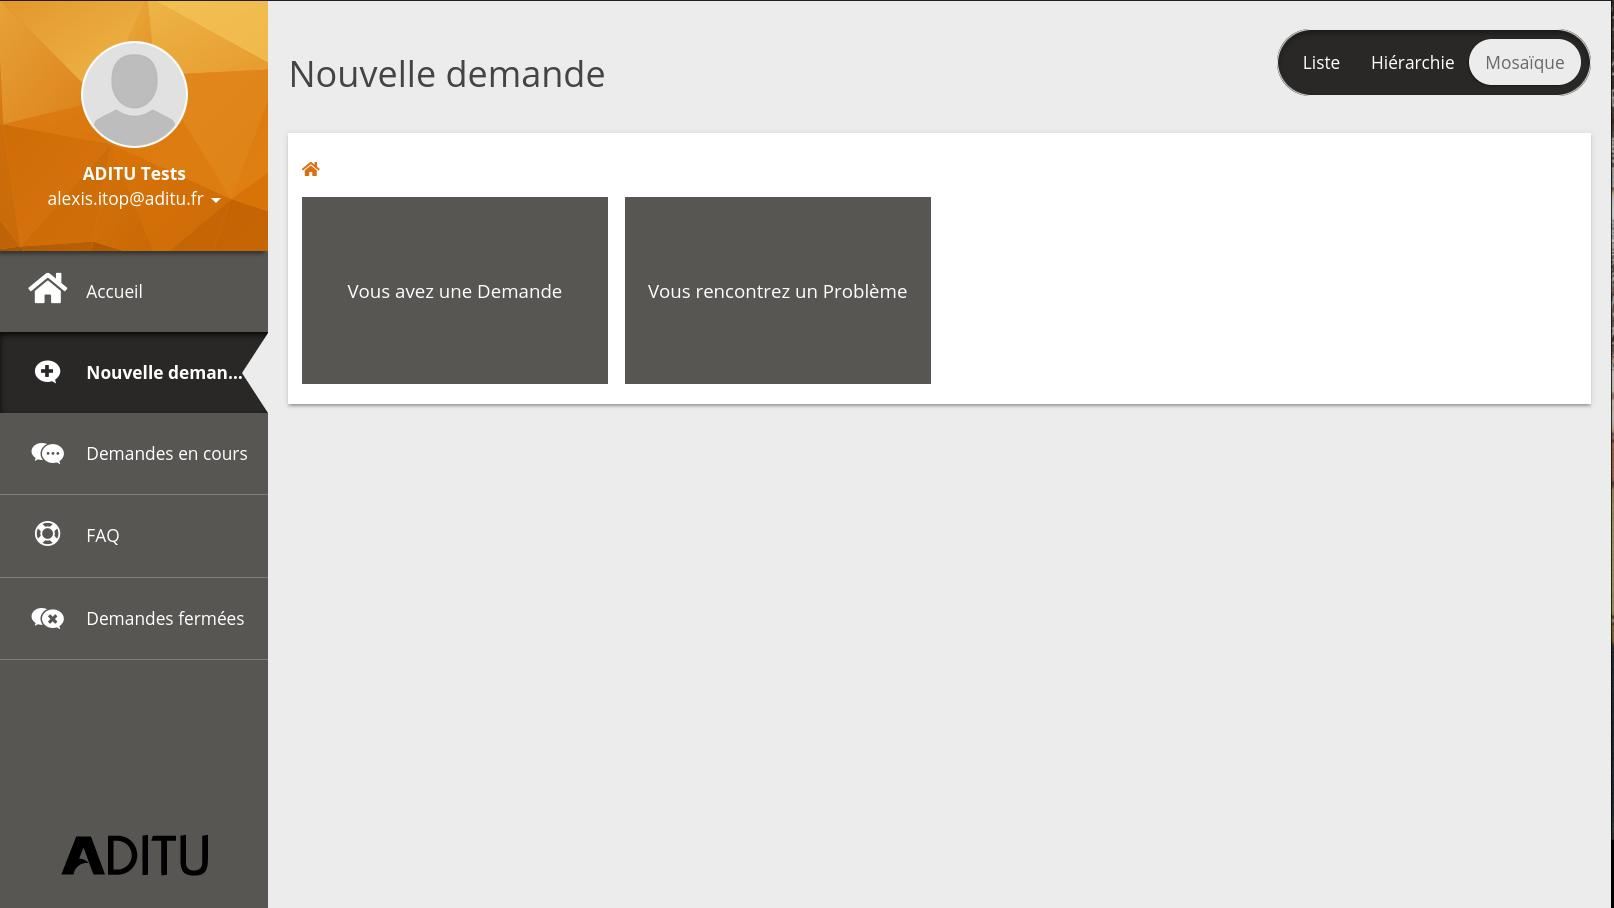
\includegraphics[width=\textwidth - \textwidth / 10]{ressources/images-itop/01.jpg}
    %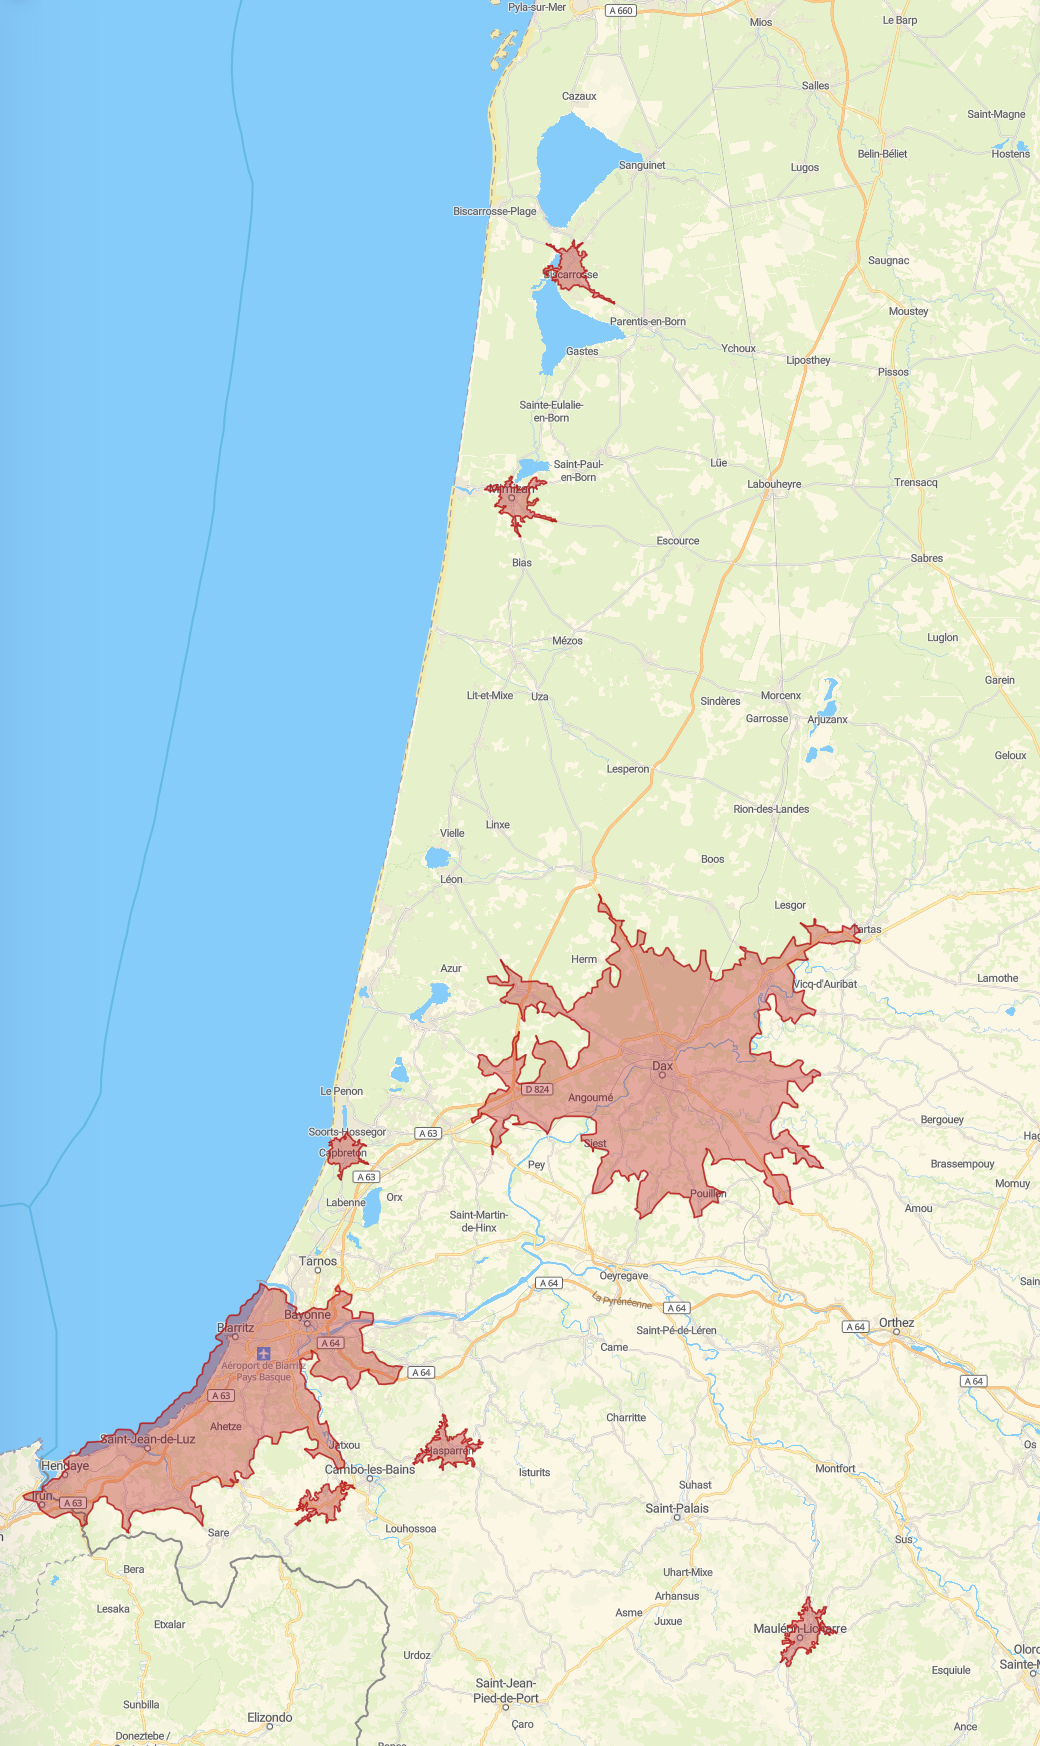
\includegraphics[scale=0.2]{zone_chalandise_aditu.png}
    \figurename
    \caption{Le client souhaite formuler une demande ou un incident}
    \label{fig:01-itop}
\end{figure}

\begin{figure}[H]
    \centering
    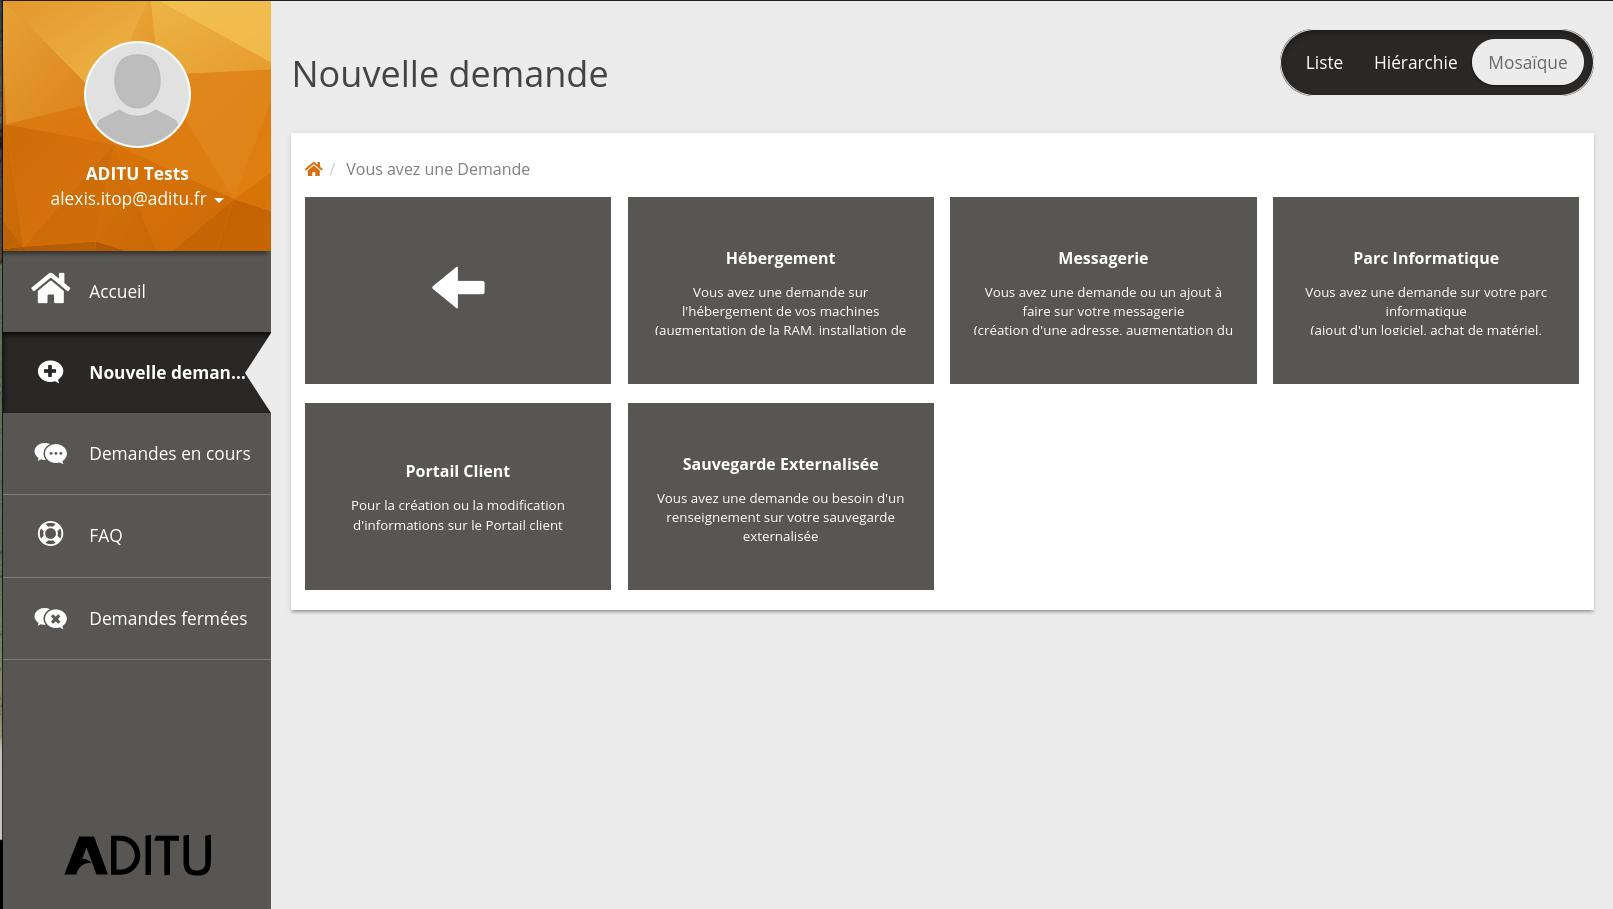
\includegraphics[width=\textwidth - \textwidth / 10]{ressources/images-itop/02.jpg}
    %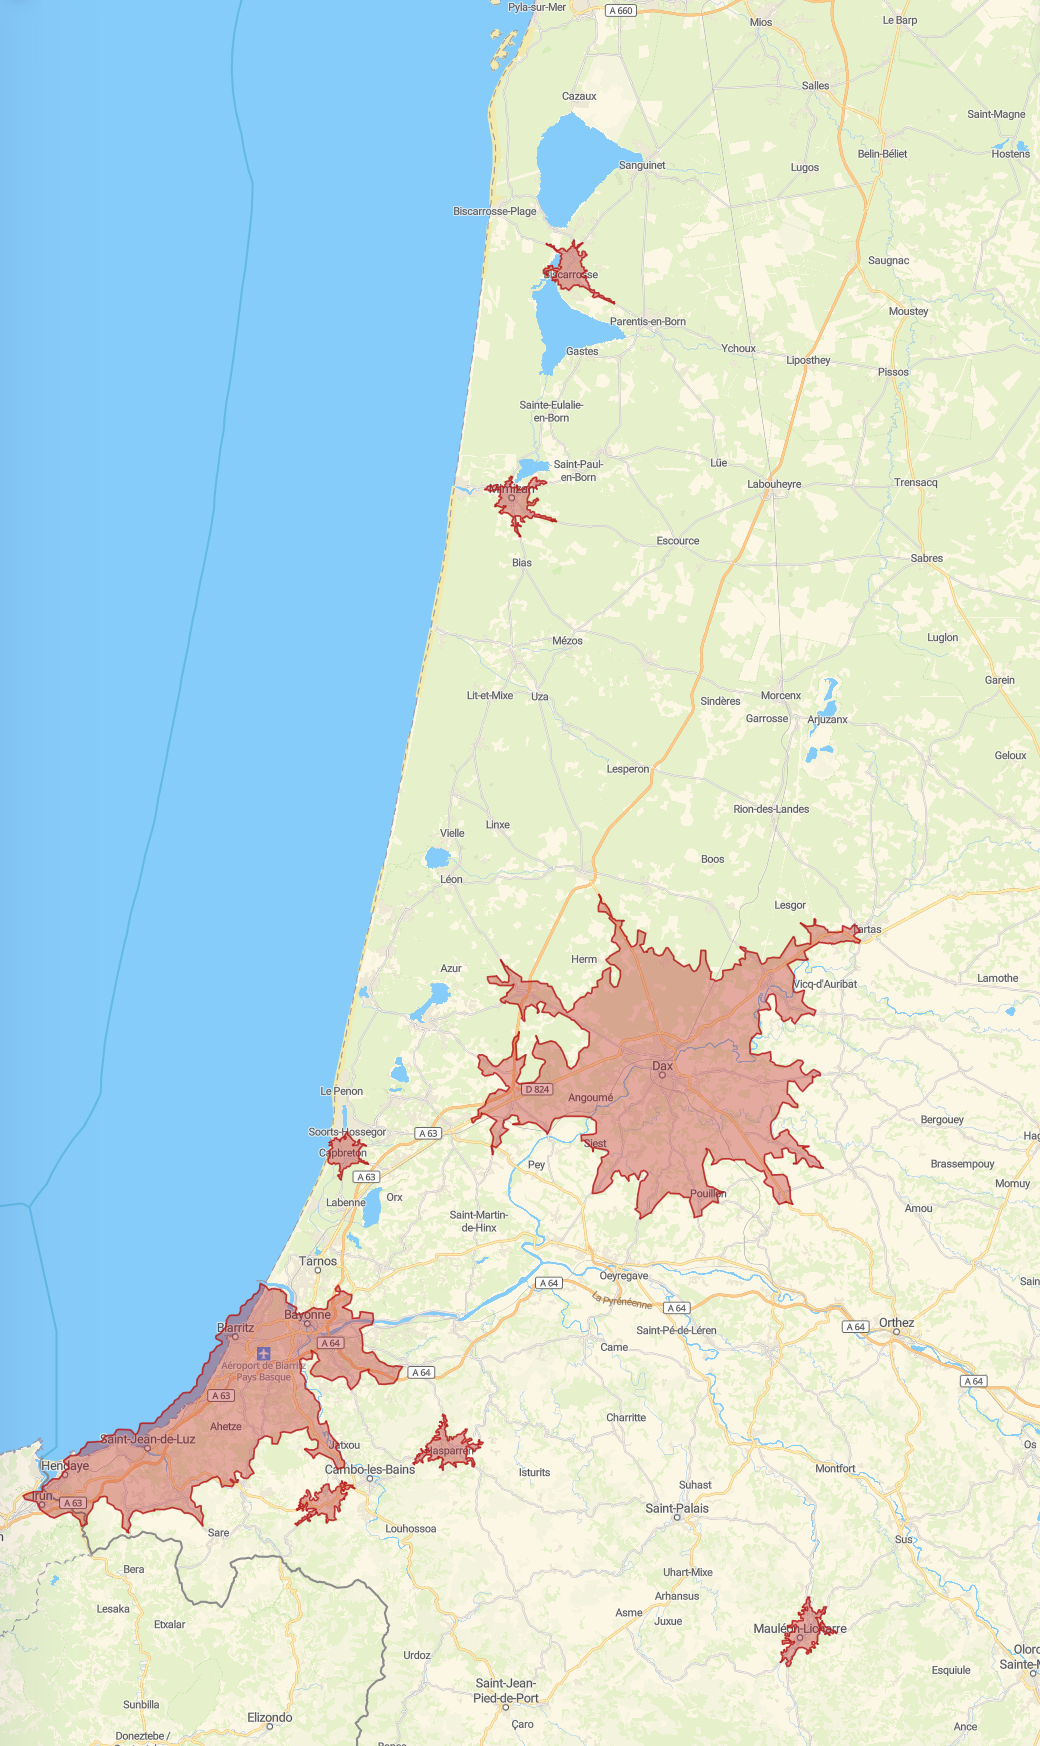
\includegraphics[scale=0.2]{zone_chalandise_aditu.png}
    \figurename
    \caption{Le client choisit le services touché par sa demande (ici, il a beaucoup de services associés)}
    \label{fig:02-itop}
\end{figure}

\subsection{Définition d'un espace d'échange d'informations}

Lors de la préparation, une discussion faisait débat sur l'applicatif : faut-il définir une FAQ \textit{Foire Aux Questions} pour les utilisateurs qui utilisent l'interface (de tout niveau) et/ou un KB \textit{Knowledge Base} pour recueillir les informations pratiques et des procédures à suivre pour certains problèmes des clients.
\\ \\
Chacun comporte ses avantages et ses inconvénients. L'équipe a décidé de garder une FAQ, car elle n'a pas à être trop régulièrement être maintenue , aussi parce qu'elle n'est pas vouée à devenir obsolète dans le temps à contrario d'une KB. Celle-ci s'adresse d'autant plus à un plus grand public, pouvant être lue par beaucoup (pas besoin de compétence techniques, pas de cas par cas...).

\begin{figure}[H]
    \centering
    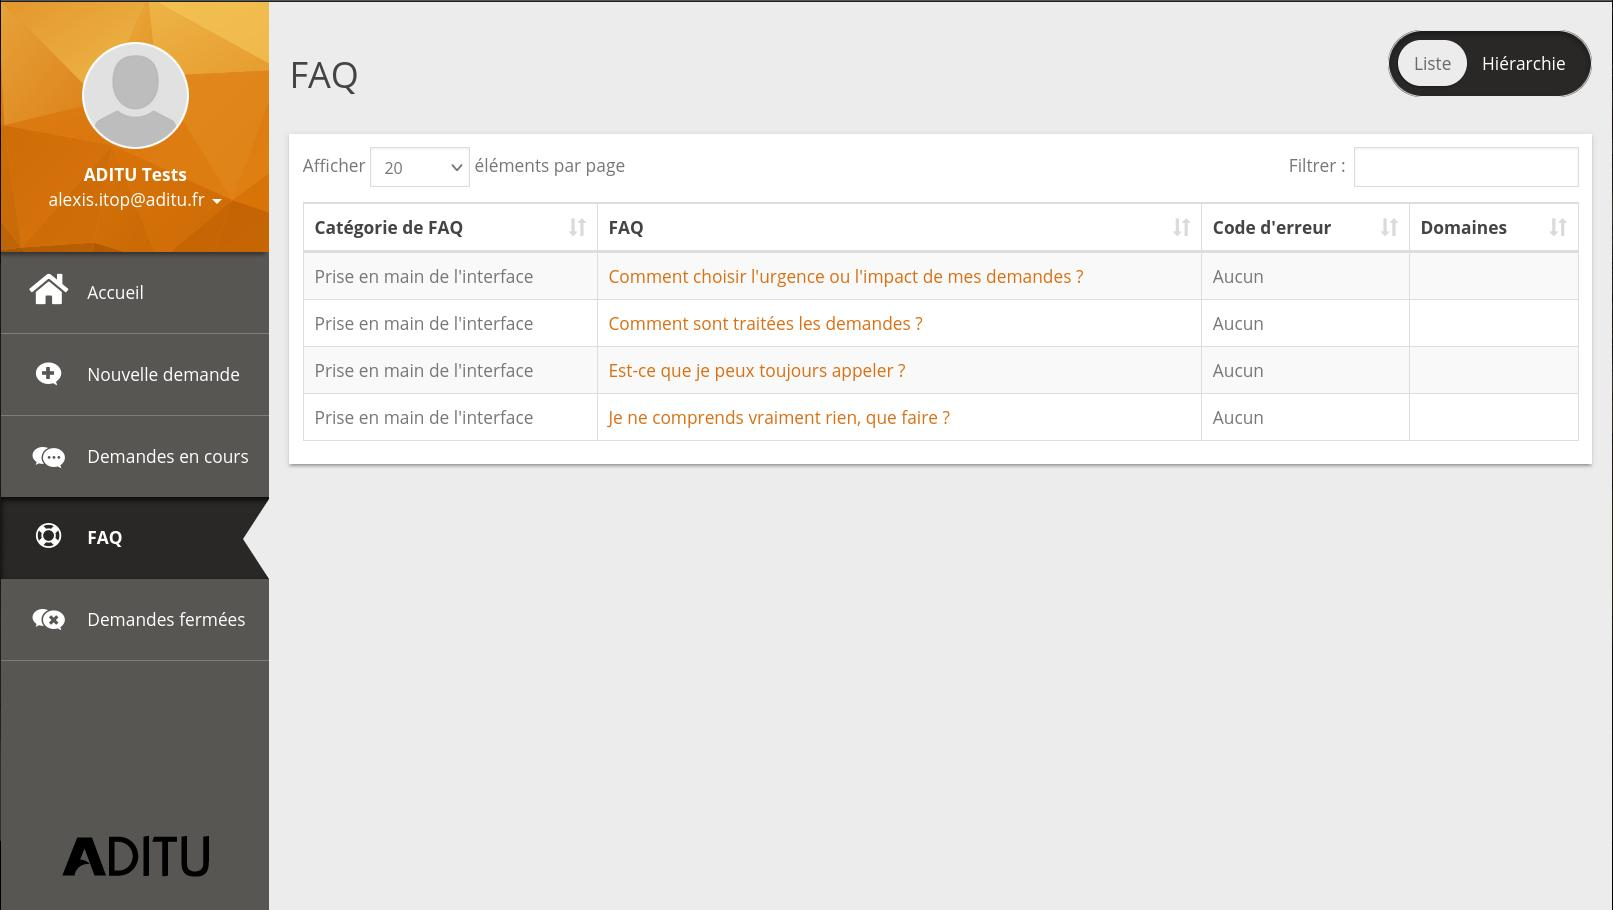
\includegraphics[width=\textwidth - \textwidth / 10]{ressources/images-itop/03.jpg}
    %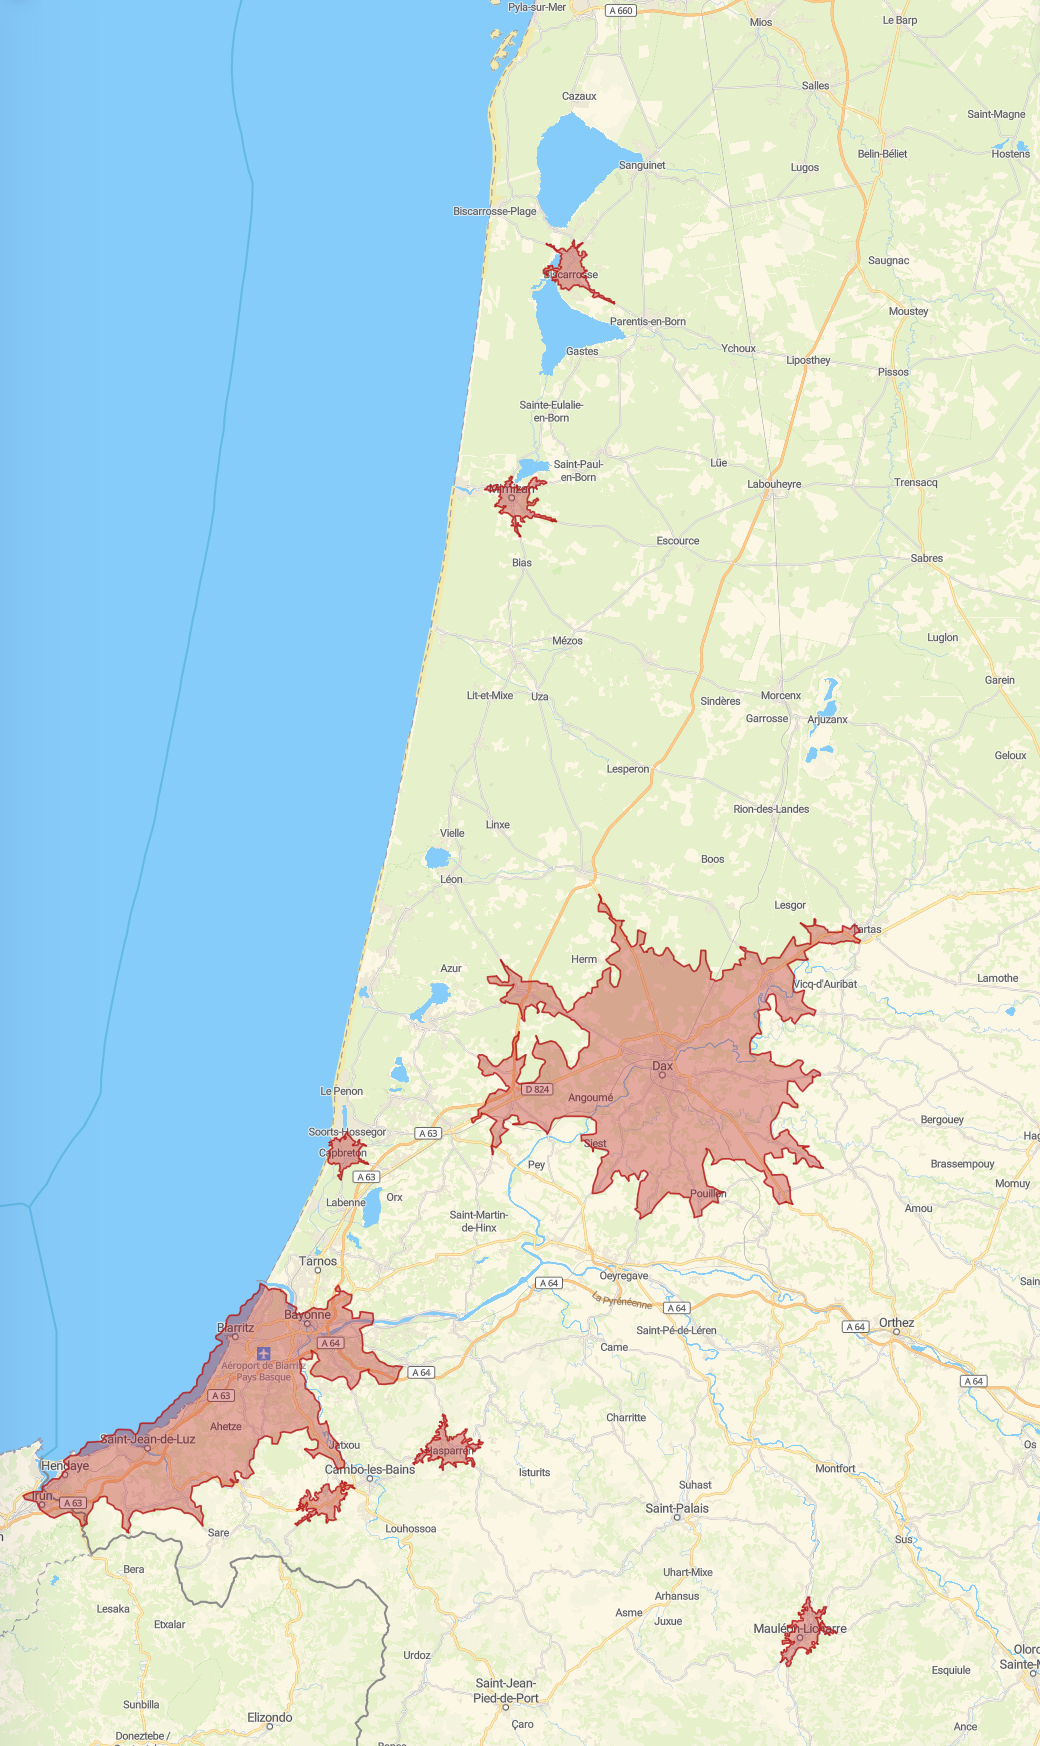
\includegraphics[scale=0.2]{zone_chalandise_aditu.png}
    \figurename
    \caption{Exemple de FAQ présentée au client}
    \label{fig:03-itop}
\end{figure}

\subsection{Application d'un test de charge}

Le dernier test appliqué fut celui d'un test de charge \textit{ou stress test} pour savoir si l'application pouvait répondre à une grande charge (attaque par déni de service, mal fonctionnement, comportement invonlontaire...).
\\ \\
Ainsi, son comportement fut testé lorsque ses ressources matérielles étaient saturées (pouvant provenir du système d'exploitation), lorsque qu'un nombre anormal de tickets sont créés voir le comportement de la base de donnée etc. (toujours attaque par deni de services par rebond sur un compte client).
\\ \\
Tous les tests ont été passés, et suite à une validation de l'équipe, la solution pourra être lancée à mon retour.